%author : berenice delcroix-oger
%colors of rainbow trees
\documentclass[border=2pt]{standalone}
\usepackage{tikz}
\usetikzlibrary{positioning, fit, shapes, arrows, calc}

\pgfdeclarelayer{bg}    % declare background layer
\pgfsetlayers{bg,main}  % set the order of the layers (main is the standard layer)

\newcommand{\coula}{0785F2}
\newcommand{\coulb}{F29F05}
\newcommand{\coulc}{F21313}
\newcommand{\could}{E6F21F}



\definecolor{bleu}{HTML}{0000FF} 
\definecolor{vert}{HTML}{39B44B}
\definecolor{rouge}{HTML}{FF0000}



\definecolor{part1}{HTML}{\coula}
\definecolor{part2}{HTML}{\coulb}
\definecolor{part3}{HTML}{\coulc}
\definecolor{part4}{HTML}{\could}

\begin{document}
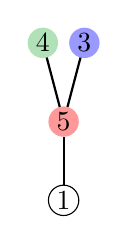
\begin{tikzpicture}[grow=up, inner sep=1pt,  outer sep=0pt, level distance=1cm, sibling distance=15pt]
\node[draw, circle] {$1$}
   child[thick]{node[circle, fill=rouge, fill opacity=0.4, text opacity=1, anchor=center] {$5$}
          child{node[circle, fill=bleu, fill opacity=0.4, text opacity=1] {$3$}}
          child{node[circle, fill=vert, fill opacity=0.4, text opacity=1] {$4$}}     
   };
\end{tikzpicture}
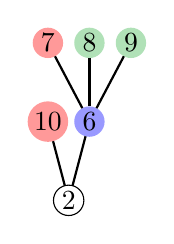
\begin{tikzpicture}[grow=up, inner sep=1pt, level distance=1cm, sibling distance=15pt,  outer sep=0pt]
\node[draw, circle] {$2$}
   child[thick]{node[circle, fill=bleu, fill opacity=0.4, text opacity=1, anchor=center] {$6$}
          child{node[circle, fill=vert, fill opacity=0.4, text opacity=1] {$9$}}
          child{node[circle, fill=vert, fill opacity=0.4, text opacity=1] {$8$}}     
          child{node[circle, fill=rouge, fill opacity=0.4, text opacity=1] {$7$}}     
   }
   child[thick]{node[circle, fill=rouge, fill opacity=0.4, text opacity=1, anchor=center] {$10$}}
;
\end{tikzpicture}

\end{document}
